\documentclass{article}
\usepackage{amsmath, amssymb, ctex, graphicx, color}
\usepackage[margin=1in]{geometry}
\usepackage{setspace} % 行距控制
\usepackage{array}
\usepackage{makecell}
\usepackage{booktabs}

\usepackage{algorithm}
\usepackage{algpseudocode}
\usepackage{xcolor}
% 把默认注释符号 ▷ 改成行尾 // 等宽紫色，并右对齐
\renewcommand{\algorithmiccomment}[1]{\hfill\texttt{\textcolor{violet}{// #1}}}
% 定义 Input / Output 关键字（默认是 Require / Ensure）
\algnewcommand\algorithmicinput{\textbf{Input:}}
\algnewcommand\algorithmicoutput{\textbf{Output:}}
\algnewcommand\Input{\item[\algorithmicinput]}
\algnewcommand\Output{\item[\algorithmicoutput]}

\usepackage{titling}\setlength{\droptitle}{-2cm} 
\title{Ch7. Gradient Descent \\ 
Section 7.4. Normalization \\
第7章-梯度下降 -- 第7.4节-归一化}
\author{《深度学习基础》课程小组}
% \date{}
 
\begin{document}
\maketitle
% \tableofcontents

\setlength{\parindent}{0pt} % 取消首行缩进
\setlength{\parskip}{1.5em} % 设置段落之间的距离

\noindent\rule{\linewidth}{0.4pt}

\section{P1}

Normalization of the variables computed during the forward pass through a neural network removes the need for the network to deal with extremely large or extremely small values. 

Although in principle the weights and biases in a neural network can adapt to whatever values the input and hidden variables take, in practice normalization can be crucial for ensuring effective training. 

Here we consider three kinds of normalization according to whether we are normalizing across the input data, across mini-batches, or across layers.

{\color{red}
翻译：

对神经网络前向传播过程中计算出的变量进行归一化，消除了网络处理极大或极小数值的需求。

虽然原则上神经网络中的权重和偏置可以适应输入和隐藏变量取的任何值，但在实践中，归一化对于确保有效的训练至关重要。

在这里，我们根据是对输入数据、小批量（mini-batches）还是跨层进行归一化，来考虑三种归一化方法。
}

{\color{blue}
问：为什么在实践中归一化对于确保有效的训练至关重要？

答：归一化在神经网络训练中至关重要，主要原因包括以下几点：

统一输入量纲，避免特征主导偏差：当输入数据各特征量纲差异巨大时（如身高1.8米 vs 血小板30万/$\mu$L），未归一化的数据会导致模型权重学习失衡。大量纲特征会主导梯度更新，使小量纲特征被忽略，影响模型对真实关系的捕捉。

加速收敛，提升训练效率：归一化使损失函数曲面更平滑，梯度方向更稳定，允许使用更大的学习率而不发散。这显著减少训练迭代次数，加快模型收敛速度。

缓解梯度消失与爆炸问题：深层网络中，未归一化的激活值可能在传播过程中指数级放大或缩小，导致梯度消失或爆炸。归一化通过控制每层输出的分布范围，维持梯度在合理区间，保障反向传播的有效性。

降低对初始化和超参数的敏感性：归一化使网络对权重初始化方式和学习率选择不那么敏感，提升了模型的鲁棒性和可复现性，便于工程实践中的调参。

支持更深网络结构的训练：Batch Normalization等技术通过稳定中间层分布，使构建和训练数十甚至上百层的深度网络成为可能，推动了现代深度学习架构的发展。

这些机制共同作用，使归一化成为确保神经网络高效、稳定、可靠训练的关键技术。
}

\noindent\rule{\linewidth}{0.4pt}

\section{P1: 7.4.1 Data normalization}

Sometimes we encounter data sets in which different input variables span very different ranges. 

For example, in health data, a patient's height might be measured in meters, such as $1.8\,\mathrm{m}$, whereas their blood platelet count might be measured in platelets per microliter, such as $300{,}000$ platelets per $\mu\mathrm{L}$. 

Such variations can make gradient descent training much more challenging. 

{\color{red}
翻译：

有时我们会遇到这样的数据集，其中不同的输入变量跨越的范围差异非常大。

例如，在健康数据中，患者的身高可能以米为单位测量，如 $1.8\,\mathrm{m}$，而其血小板计数可能以每微升血小板数为单位测量，如 $300{,}000$ 个血小板每 $\mu\mathrm{L}$。

这种差异会使梯度下降训练变得更加困难。
}

Consider a single-layer regression network with two weights in which the two corresponding input variables have very different ranges. 

Changes in the value of one of the weights produce much larger changes in the output, and hence in the error function, than would similar changes in the other weight. 

This corresponds to an error surface with very different curvatures along different axes as illustrated in Figure~7.3.

{\color{red}
翻译：

考虑一个具有两个权重的单层回归网络，其中两个相应的输入变量具有非常不同的范围。

其中一个权重的值发生变化所引起的输出（以及因此引起的误差函数）的变化，要比另一个权重发生类似变化所引起的变化大得多。

这对应于一个沿不同轴具有非常不同曲率的误差曲面，如图~7.3所示。

}

\begin{figure}[ht]\centering
    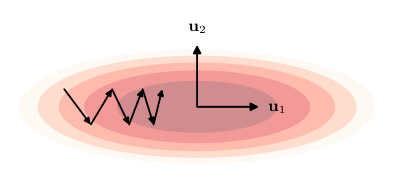
\includegraphics[width=0.4\textwidth]{../ch07-3/figure7-3.png}
    \caption{图7.3: 误差曲面沿着不同的轴有非常不同的曲率}
\end{figure}

\noindent\rule{\linewidth}{0.4pt}

\section{P3}

For continuous input variables, it can therefore be very beneficial to re-scale the input values so that they span similar ranges. 

This is easily done by first evaluating the mean and variance of each input:
\begin{align}
    \mu_i &= \frac{1}{N} \sum_{n=1}^N x_{ni} \tag{7.48} \\
    \sigma_i^2 &= \frac{1}{N} \sum_{n=1}^N (x_{ni} - \mu_i)^2, \tag{7.49}
\end{align}
which is a calculation that is performed once, before any training is started. 

The input values are then re-scaled using
\begin{equation}
    \widetilde{x}_{ni} = \frac{x_{ni} - \mu_i}{\sigma_i} \tag{7.50}
\end{equation}
so that the re-scaled values $\{\widetilde{x}_{ni}\}$ have zero mean and unit variance. 

Note that the same values of $\mu_i$ and $\sigma_i$ must be used to pre-process any development, validation, or test data to ensure that all inputs are scaled in the same way. 

{\color{red}
翻译：

因此，对于连续的输入变量，重新缩放输入值使其跨越相似的范围是非常有益的。

这可以通过首先计算每个输入的均值和方差来轻松完成：
\begin{align}
    \mu_i &= \frac{1}{N} \sum_{n=1}^N x_{ni} \tag{7.48} \\
    \sigma_i^2 &= \frac{1}{N} \sum_{n=1}^N (x_{ni} - \mu_i)^2, \tag{7.49}
\end{align}
这是一次性计算，在任何训练开始之前进行。

然后使用以下公式重新缩放输入值
\begin{equation}
    \widetilde{x}_{ni} = \frac{x_{ni} - \mu_i}{\sigma_i} \tag{7.50}
\end{equation}
使得重新缩放后的值 $\{\widetilde{x}_{ni}\}$ 具有零均值和单位方差。

请注意，必须使用相同的 $\mu_i$ 和 $\sigma_i$ 值来预处理任何开发集、验证集或测试集数据，以确保所有输入都以相同的方式进行缩放。
}

Input data normalization is illustrated in Figure~7.7.

Figure 7.7 Caption: Illustration of the effect of input data normalization. 

The red circles show the original data points for a data set with two variables. 

The blue crosses show the data set after normalization such that each variable now has zero mean and unit variance across the data set.

{\color{red}
输入数据归一化如图~7.7所示。图 7.7 说明：输入数据归一化效果的示意图。红色圆圈显示了具有两个变量的数据集的原始数据点。蓝色叉号显示了归一化后的数据集，此时每个变量在整个数据集中现在都具有零均值和单位方差。

}

\begin{figure}[ht]\centering
    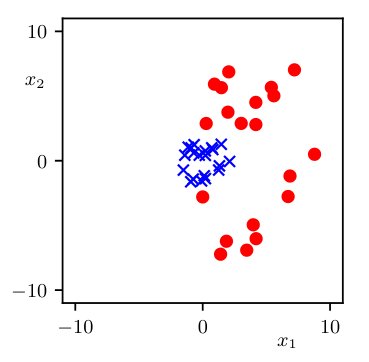
\includegraphics[width=0.4\textwidth]{figure7-7.png}
    \caption{图7.7: 蓝色数据是红色数据的归一化}
\end{figure}

{\color{blue}
问：开发集、验证集、测试集数据的区别是什么？

答：在机器学习中，开发集、验证集和测试集是用于模型训练与评估的三个关键数据集，它们各自承担不同的功能，共同确保模型的泛化能力和可靠性。

开发集（Development Set）：也称为验证集（Validation Set），主要用于在模型训练过程中调整超参数、选择模型架构或决定是否停止训练。它帮助开发者在训练阶段评估模型的初步泛化能力，从而指导模型优化方向。

验证集（Validation Set）：与开发集功能基本一致，常用于交叉验证或独立评估模型在不同配置下的表现。它在训练过程中被反复使用，以监控模型是否过拟合或欠拟合，并据此调整学习率、层数、神经元数量等超参数。

测试集（Test Set）：用于最终评估模型的泛化性能，必须在模型完全训练和调优完成后使用。测试集的数据在整个训练和调参过程中不可见，以确保评估结果的客观性和无偏性。它模拟真实世界中模型面对新数据时的表现，是衡量模型最终效果的金标准。

这三者必须保持数据分布的一致性，且不能相互重叠。在实际项目中，若训练集与测试集数据来源不同（如训练用网络图片，测试用手机拍摄图），可能导致模型在部署时性能骤降，因此需特别注意数据匹配问题。

% 这三个集合的划分比例其实很有讲究，需要我讲讲怎么根据数据量大小来合理分配吗？
}


\noindent\rule{\linewidth}{0.4pt}

\section{P4: 7.4.2 Batch normalization}

We have seen the importance of normalizing the input data, and we can apply similar reasoning to the variables in each hidden layer of a deep network. 

If there is wide variation in the range of activation values in a particular hidden layer, then normalizing those values to have zero mean and unit variance should make the learning problem easier for the next layer. 

However, unlike normalization of the input values, which can be done once prior to the start of training, normalization of the hidden-unit values will need to be repeated during training every time the weight values are updated. 

This is called \emph{batch normalization} (Ioffe and Szegedy, 2015).


{\color{red}
翻译：

我们已经看到了归一化输入数据的重要性，同样的逻辑也可以应用到深层网络中每个隐藏层的变量上。

如果某个特定隐藏层中激活值的范围存在很大的差异，那么将这些值归一化为零均值和单位方差，应该会使下一层的学习问题变得更容易。

然而，与可以在训练开始前一次性完成的输入值归一化不同，隐藏单元值的归一化在训练过程中每次更新权重值时都需要重复进行。

这被称为批归一化（batch normalization）（Ioffe and Szegedy, 2015）。

}

\noindent\rule{\linewidth}{0.4pt}

\section{P5}

A further motivation for batch normalization arises from the phenomena of \emph{vanishing gradients} and \emph{exploding gradients}, which occur when we try to train very deep neural networks. 

From the chain rule of calculus, the gradient of an error function $E$ with respect to a parameter in the first layer of the network is given by
\begin{equation}
    \frac{\partial E}{\partial w_i} = 
    \sum_m \cdots \sum_l \sum_j 
    \frac{\partial z_m^{(1)}}{\partial w_i}
    \cdots
    \frac{\partial z_j^{(K)}}{\partial z_l^{(K-1)}}
    \frac{\partial E}{\partial z_j^{(K)}} \tag{7.51}
\end{equation}
where $z_j^{(k)}$ denotes the activation of node $j$ in layer $k$, and each of the partial derivatives on the right-hand side of (7.51) represents the elements of the Jacobian matrix for that layer. 

The product of a large number of such terms will tend towards $0$ if most of them have a magnitude $<1$ and will tend towards $\infty$ if most of them have a magnitude $>1$. 

Consequently, as the depth of a network increases, error function gradients can tend to become either very large or very small. 

Batch normalization largely resolves this issue.

{\color{red}
翻译：

批归一化的另一个动机源于\emph{梯度消失}（\emph{vanishing gradients}）和\emph{梯度爆炸}（\emph{exploding gradients}）现象，这些现象在我们尝试训练极深的神经网络时会出现。

根据微积分中的链式法则，误差函数 $E$ 对网络第一层某个参数的梯度为：
\begin{equation}
    \frac{\partial E}{\partial w_i} = 
    \sum_m \cdots \sum_l \sum_j 
    \frac{\partial z_m^{(1)}}{\partial w_i}
    \cdots
    \frac{\partial z_j^{(K)}}{\partial z_l^{(K-1)}}
    \frac{\partial E}{\partial z_j^{(K)}} \tag{7.51}
\end{equation}
其中，$z_j^{(k)}$ 表示第 $k$ 层中节点 $j$ 的激活值，等式 (7.51) 右侧的每个偏导数都代表该层雅可比矩阵（Jacobian matrix）的元素。

如果其中大多数项的幅值 $<1$，那么大量这样的项相乘将趋于 $0$；如果大多数项的幅值 $>1$，乘积将趋于 $\infty$。

因此，随着网络深度的增加，误差函数的梯度往往会变得非常大或非常小。

批归一化在很大程度上解决了这个问题。
}

\noindent\rule{\linewidth}{0.4pt}

\section{P6}

To see how batch normalization is defined, consider a specific layer within a multi-layer network. 

Each hidden unit in that layer computes a nonlinear function of its input pre-activation $z_i = h(a_i)$, and so we have a choice of whether to normalize the pre-activation values $a_i$ or the activation values $z_i$. 

In practice, either approach may be used, and here we illustrate the procedure by normalizing the pre-activations. 

Because weight values are updated after each mini-batch of examples, we apply the normalization to each mini-batch. 

Specifically, for a mini-batch of size $K$, we define
\begin{align}
    \mu_i &= \frac{1}{K} \sum_{n=1}^K a_{ni} \tag{7.52} \\
    \sigma_i^2 &= \frac{1}{K} \sum_{n=1}^K (a_{ni} - \mu_i)^2 \tag{7.53} \\
    \widehat{a}_{ni} &= \frac{a_{ni} - \mu_i}{\sqrt{\sigma_i^2 + \delta}} \tag{7.54}
\end{align}
where the summations over $n = 1, \dots, K$ are taken over the elements of the mini-batch. 

Here $\delta$ is a small constant, introduced to avoid numerical issues in situations where $\sigma_i^2$ is small.

{\color{red}
翻译：

为了了解批归一化是如何定义的，我们考虑多层网络中的一个特定层。

该层中的每个隐藏单元都会计算其输入预激活值的非线性函数 $z_i = h(a_i)$，因此我们可以选择是对预激活值 $a_i$ 进行归一化，还是对激活值 $z_i$ 进行归一化。

在实际应用中，这两种方法都可以使用，这里我们通过归一化预激活值来说明整个过程。

由于权重值是在每个小批量（mini-batch）样本之后更新的，因此我们对每个小批量应用归一化。

具体来说，对于大小为 $K$ 的小批量，我们定义：
\begin{align}
    \mu_i &= \frac{1}{K} \sum_{n=1}^K a_{ni} \tag{7.52} \\
    \sigma_i^2 &= \frac{1}{K} \sum_{n=1}^K (a_{ni} - \mu_i)^2 \tag{7.53} \\
    \widehat{a}_{ni} &= \frac{a_{ni} - \mu_i}{\sqrt{\sigma_i^2 + \delta}} \tag{7.54}
\end{align}
其中，对 $n = 1, \dots, K$ 的求和是在小批量的元素上进行的。

这里的 $\delta$ 是一个小常数，引入它是为了避免在 $\sigma_i^2$ 很小的情况下出现数值计算问题。

}

\noindent\rule{\linewidth}{0.4pt}

\section{P7}

By normalizing the pre-activations in a given layer of the network, we reduce the number of degrees of freedom in the parameters of that layer and hence we reduce its representational capability. 

We can compensate for this by re-scaling the pre-activations of the batch to have mean $\beta_i$ and standard deviation $\gamma_i$ using
\begin{equation}
    \widetilde{a}_{ni} = \gamma_i \widehat{a}_{ni} + \beta_i \tag{7.55}
\end{equation}
where $\beta_i$ and $\gamma_i$ are adaptive parameters that are learned by gradient descent jointly with the weights and biases of the network. 

These learnable parameters represent a key difference compared to input data normalization.

{\color{red}
翻译：

通过对网络中给定层的预激活值进行归一化，我们减少了该层参数的自由度，从而降低了它的表示能力。

我们可以通过使用以下公式重新缩放该批次的预激活值，使其具有均值 $\beta_i$ 和标准差 $\gamma_i$，以此来弥补这一损失：
\begin{equation}
    \widetilde{a}_{ni} = \gamma_i \widehat{a}_{ni} + \beta_i \tag{7.55}
\end{equation}
其中，$\beta_i$ 和 $\gamma_i$ 是自适应参数，它们与网络的权重和偏置一起通过梯度下降进行联合学习。

这些可学习的参数代表了批归一化与输入数据归一化之间的一个关键区别。
}

{\color{blue}
问：批归一化与输入数据归一化之间的区别有哪些？

答：结合刚才翻译的原文内容以及深度学习的基础理论，批归一化（Batch Normalization）与输入数据归一化（Input Data Normalization）的核心区别主要体现在以下几个方面：

1. 归一化的对象与位置不同

输入数据归一化：仅针对神经网络的输入层变量进行。它通常在训练开始前作为数据预处理步骤一次性完成。

批归一化：针对深层网络中每一个隐藏层的变量（如预激活值或激活值）进行。它作为一个独立的层嵌入在网络结构中，在训练和推理过程中持续发挥作用。

2. 是否包含可学习的参数（最核心的区别）

输入数据归一化：通常将数据强制缩放为固定的零均值和单位方差。这个过程是固定的，不包含任何需要通过梯度下降学习的参数。

批归一化：在强制归一化为零均值和单位方差后，引入了两个可学习的自适应参数 $\beta_i$（均值）和 $\gamma_i$（标准差）。网络可以通过梯度下降自动学习并恢复或调整数据的分布。正如原文所述，这弥补了强制归一化带来的“表示能力下降”的问题。

3. 统计量的计算时机与方式不同

输入数据归一化：均值和方差是基于整个训练数据集计算的，在训练开始前一次性计算完毕，后续不再改变。

批归一化：均值和方差是基于当前训练的小批量（mini-batch）动态计算的。因为权重在每次小批量更新后都会改变，所以隐藏层的分布也在不断变化，必须重复进行归一化计算。

4. 推理（测试）阶段的处理方式不同

输入数据归一化：推理时直接使用训练前计算好的固定均值和方差对新数据进行缩放即可。

批归一化：推理时通常没有小批量数据，无法实时计算均值和方差。因此，需要在训练阶段通过移动平均（moving averages）记录各层均值和方差的估计值，并在推理阶段使用这些全局估计值进行处理。

5. 解决的痛点不同

输入数据归一化：主要解决输入特征量纲不一致（如身高与血小板计数）导致的梯度下降困难、收敛慢的问题。

批归一化：除了让下一层的学习更容易外，更关键的是缓解了深层网络中因链式法则连乘导致的梯度消失和梯度爆炸问题，使得训练极深的网络成为可能。

% 要不要接着看训练和推理阶段处理方式的差异，以及移动平均的计算公式？


}

\noindent\rule{\linewidth}{0.4pt}

\section{P8}

It might appear that the transformation (7.55) has simply undone the effect of the batch normalization since the mean and variance can now adapt to arbitrary values again. 

However, the crucial difference is in the way the parameters evolve during training. 

For the original network, the mean and variance across a mini-batch are determined by a complex function of all the weights and biases in the layer, whereas in the representation given by (7.55), they are determined directly by independent parameters $\beta_i$ and $\gamma_i$, which turn out to be much easier to learn during gradient descent.

{\color{red}
翻译：

这看起来似乎使得变换 (7.55) 抵消了批归一化的效果，因为均值和方差现在又可以适应任意值了。

然而，关键的区别在于参数在训练过程中的演变方式。

对于原始网络，一个小批量数据上的均值和方差是由该层所有的权重和偏置通过一个复杂的函数决定的；而在由 (7.55) 给出的表示中，均值和方差直接由独立的参数 $\beta_i$ 和 $\gamma_i$ 决定，事实证明，在梯度下降过程中这些参数要容易学习得多。

% 要不要接着看训练和推理阶段处理方式的差异，以及移动平均的计算公式？
}

{\color{blue}
问：“关键的区别在于参数在训练过程中的演变方式。如何理解这句话？

答：这句话的核心在于探讨：在神经网络中，我们如何控制中间层数据的分布（均值和方差）？

为了让你透彻理解，我们需要对比“没有引入 $\beta, \gamma$ 的原始网络”和“引入 $\beta, \gamma$ 后的批归一化网络”在训练时的本质差异：

1. 原始网络中的“被动演变”（间接控制）

在没有批归一化的原始网络中，某一层输出的均值和方差并不是独立存在的，而是由该层所有的权重（$W$）和偏置（$b$）共同决定的。

复杂的耦合关系：如果你想要改变这一层输出的均值，你实际上是在改变网络中的 $W$ 和 $b$。但问题是，$W$ 和 $b$ 的首要任务是“拟合数据特征”和“最小化误差”。

优化的冲突：当梯度下降更新 $W$ 和 $b$ 时，数据分布的改变只是这个复杂数学函数的“副产物”。如果改变分布对降低误差没有直接帮助，网络就不会去调整它。这导致中间层数据的分布极其不稳定，随着前面的层不断更新，后面的层看到的分布一直在剧烈变化（即内部协变量偏移）。

2. 批归一化中的“主动演变”（直接控制）

引入 $\beta_i$ 和 $\gamma_i$ 之后，情况发生了根本性的改变：

解耦与独立：我们将“控制数据分布”的任务从 $W$ 和 $b$ 中剥离了出来，交给了专门的参数 $\beta_i$（控制均值）和 $\gamma_i$（控制方差）。

独立的优化通道：在反向传播时，损失函数对 $\beta_i$ 和 $\gamma_i$ 有直接的梯度。这意味着，如果当前层的均值或方差偏离了最有利于学习的范围，梯度下降会直接、独立地去更新这两个参数，把分布“拉”回正轨，而不需要去绕弯子修改 $W$ 和 $b$。

总结-打个比方：

原始网络就像是你试图通过踩油门和打方向盘（改变 $W, b$）来顺便控制车内的空调温度。这非常困难，因为你的主要任务是开车，很难精准且独立地控制温度。

批归一化则是给汽车单独装了一个空调温度旋钮（$\beta, \gamma$）。现在你可以一边让司机专心开车，一边通过旋钮直接、独立地调节温度。

因此，“参数在训练过程中的演变方式”的区别就在于：一个是间接且高度耦合的被动演变，另一个是直接且独立的主动优化。这就是为什么批归一化能让训练变得更容易的原因。

% 理解了原理，要不要接着看训练和推理阶段处理方式的差异，以及移动平均的计算公式？

}

\noindent\rule{\linewidth}{0.4pt}

\section{P9}

Equations (7.52)--(7.55) describe a transformation of the variables that is differentiable with respect to the learnable parameters $\beta_i$ and $\gamma_i$. 

This can be viewed as an additional layer in the neural network, and so each standard hidden layer can be followed by a batch normalization layer. 

The structure of the batch-normalization process is illustrated in Figure~7.8.

Figure 7.8 Caption: Illustration of batch normalization and layer normalization in a neural network. 

In batch normalization, shown in (a), the mean and variance are computed across the mini-batch separately for each hidden unit. 

In layer normalization, shown in (b), the mean and variance are computed across the hidden units separately for each data point.

\begin{figure}[ht]\centering
    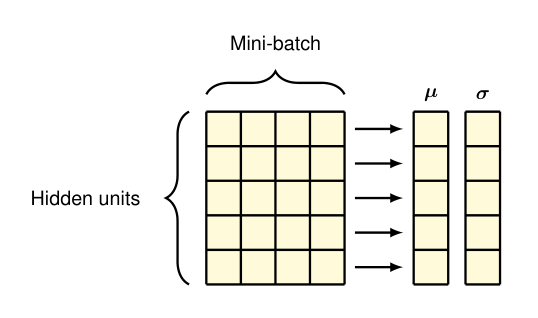
\includegraphics[width=0.4\textwidth]{figure7-8-a.png}
    \caption{图7-8-a: 批量归一化：对每个隐藏单元进行小批量归一化}
\end{figure}

{\color{red}
翻译：

公式 (7.52) 至 (7.55) 描述了一种变量的变换，该变换关于可学习参数 $\beta_i$ 和 $\gamma_i$ 是可微的。

这可以被视为神经网络中的一个附加层，因此可以在每个标准隐藏层之后跟一个批归一化层。

批归一化过程的结构如图~7.8所示。

图 7.8 说明：神经网络中批归一化和层归一化的示意图。

在 (a) 所示的批归一化中，均值和方差是针对每个隐藏单元分别跨小批量（mini-batch）计算的。

在 (b) 所示的层归一化中，均值和方差是针对每个数据点分别跨隐藏单元计算的。

% 这段话引出了层归一化（Layer Normalization）的概念，要不要接着看层归一化的具体公式和它与批归一化的对比？
}

{\color{blue}
问：公式 (7.52) 至 (7.55) 描述了一种变量的变换，该变换关于可学习参数 $\beta_i$ 和 $\gamma_i$ 是可微的。如何理解这句话？

答：这句话是理解批归一化（Batch Normalization）为何能融入神经网络训练体系的数学基石。

我们可以将这句话拆解为两个核心概念来理解：

1. 什么是“可微的（Differentiable）”？

在神经网络中，我们依赖梯度下降算法来更新参数。这个算法的前提是：损失函数对参数的求导（即计算梯度）必须是存在的、连续的。

如果公式 (7.52) 到 (7.55) 中的数学操作（如求均值、方差、加减乘除等）是不可微的（比如包含阶跃函数或取整操作），那么梯度在反向传播时就会断裂，网络就无法通过误差来指导参数的更新。

幸运的是，这几步操作全都是平滑的数学运算，因此梯度可以毫无阻碍地穿过它们。

2. 为什么要强调“关于可学习参数 $\beta_i$ 和 $\gamma_i$”？

在公式 (7.52) 和 (7.53) 中，均值 $\mu_i$ 和方差 $\sigma_i^2$ 是根据当前小批量数据动态计算出来的，它们不是模型参数，不能直接通过梯度下降来更新。

但是，公式 (7.55) $\widetilde{a}_{ni} = \gamma_i \widehat{a}_{ni} + \beta_i$ 引入了 $\beta_i$ 和 $\gamma_i$。这句话强调“关于它们是可微的”，意味着：

存在明确的优化路径：在反向传播时，损失函数可以明确地计算出 $\frac{\partial E}{\partial \beta_i}$ 和 $\frac{\partial E}{\partial \gamma_i}$。

赋予网络“自适应调节”的能力：因为可以求导，网络就能知道：如果当前层的均值偏大，$\beta_i$ 应该减小还是增大？如果方差太小，$\gamma_i$ 应该放大还是缩小？通过梯度下降，$\beta_i$ 和 $\gamma_i$ 就能自动寻找并收敛到最有利于学习的数值。

3. 为什么“可以被视为一个附加层”？

正因为这个变换过程是完全可微的，并且包含了可学习的参数，它在数学本质和工程实现上，与普通的隐藏层（如全连接层、卷积层）没有任何区别。

在代码实现中（如 PyTorch 或 TensorFlow），你只需要像添加普通层一样，在标准隐藏层后面加一行 `BatchNorm1d()` 或 `BatchNorm2d()`。

在反向传播时，框架会自动计算并更新其中的 $\beta$ 和 $\gamma$。

总结来说：这句话的意思是，批归一化不仅是一个数据预处理步骤，它本身就是一个数学上合法、支持梯度反向传播的神经网络层。正是这种“可微性”，让 $\beta$ 和 $\gamma$ 能够与网络的权重 $W$ 和偏置 $b$ 一起，在训练过程中被端到端地联合优化。

% 要不要接着看训练和推理阶段处理方式的差异，以及移动平均的计算公式？
}

\noindent\rule{\linewidth}{0.4pt}

\section{P10}

Once the network is trained and we want to make predictions on new data, we no longer have the training mini-batches available, and we cannot determine a mean and variance from just one data example. 

To solve this, we could in principle evaluate $\mu_i$ and $\sigma_i^2$ for each layer across the whole training set after we have made the final update to the weights and biases. 

However, this would involve processing the whole data set just to evaluate these quantities and is therefore usually too expensive. 

Instead, we compute moving averages throughout the training phase:
\begin{align}
    \overline{\mu}_i^{(\tau)} &= \alpha \overline{\mu}_i^{(\tau-1)} + (1-\alpha) \mu_i \tag{7.56} \\
    \overline{\sigma}_i^{(\tau)} &= \alpha \overline{\sigma}_i^{(\tau-1)} + (1-\alpha) \sigma_i \tag{7.57}
\end{align}
where $0 \leq \alpha \leq 1$. 

These moving averages play no role during training but are used to process new data points during the inference phase.

{\color{red}
翻译：

一旦网络训练完成，我们需要对新数据进行预测时，就不再拥有训练时的小批量（mini-batch）数据了，而且我们也无法仅凭单个数据样本来确定均值和方差。

为了解决这个问题，原则上我们可以在对权重和偏置进行最后一次更新后，针对整个训练集计算每一层的 $\mu_i$ 和 $\sigma_i^2$。

然而，这需要对整个数据集进行处理以计算这些统计量，因此通常计算代价过于高昂。

作为替代，我们在整个训练阶段计算移动平均值：
\begin{align}
    \overline{\mu}_i^{(\tau)} &= \alpha \overline{\mu}_i^{(\tau-1)} + (1-\alpha) \mu_i \tag{7.56} \\
    \overline{\sigma}_i^{(\tau)} &= \alpha \overline{\sigma}_i^{(\tau-1)} + (1-\alpha) \sigma_i \tag{7.57}
\end{align}
其中 $0 \leq \alpha \leq 1$。

这些移动平均值在训练过程中不起任何作用，但在推理（inference）阶段用于处理新的数据点。

% 要不要接着看层归一化（Layer Normalization）的公式和它与批归一化的对比？
}

\noindent\rule{\linewidth}{0.4pt}

\section{P11}

Although batch normalization is very effective in practice, there is uncertainty as to why it works so well. 

Batch normalization was originally motivated by noting that updates to weights in earlier layers of the network change the distribution of values seen by later layers, a phenomenon called \emph{internal covariate shift}. 

However, later studies (Santurkar et al., 2018) suggest that covariate shift is not a significant factor and that the improved training results from an improvement in the smoothness of the error function landscape.

{\color{red}
翻译：

尽管批归一化在实践中非常有效，但关于它为何能发挥如此出色作用的内在原因，目前仍存在一定的不确定性。

批归一化最初的设计动机，是观察到了这样一个现象：网络中较早层的权重更新，会改变后续层所接收到的数值分布，这一现象被称为内部协变量偏移（internal covariate shift）。

然而，后续的研究（Santurkar 等人，2018年）表明，协变量偏移并不是一个关键因素，训练效果的提升实际上源于误差函数曲面（error function landscape）平滑度的改善。

% 接下来就是本节最后一个小节：层归一化（Layer Normalization）了，要不要继续看它的翻译？
}

\noindent\rule{\linewidth}{0.4pt}

\section{P12: 7.4.3 Layer normalization}

With batch normalization, if the batch size is too small then the estimates of the mean and variance become too noisy. 

Also, for very large training sets, the mini-batches may be split across different GPUs, making global normalization across the mini-batch inefficient. 

An alternative to normalizing across examples within a mini-batch for each hidden unit separately is to normalize across the hidden-unit values for each data point separately. 

This is known as \emph{layer normalization} (Ba, Kiros, and Hinton, 2016). 

It was introduced in the context of recurrent neural networks where the distributions change after each time step making batch normalization infeasible. 

However, it is useful in other architectures such as transformer networks.

{\color{red}
翻译：

在使用批归一化时，如果小批量（mini-batch）的尺寸过小，均值和方差的估计就会变得过于嘈杂（不稳定）。

此外，对于非常大的训练集，小批量数据可能会被分配到不同的 GPU 上进行计算，这使得跨整个小批量进行全局归一化的效率变得很低。

一种替代方案是：不再为每个隐藏单元单独跨小批量内的样本进行归一化，而是针对每个数据点，单独跨该层的所有隐藏单元值进行归一化。

这种方法被称为层归一化（Layer normalization）（Ba, Kiros, and Hinton, 2016）。

它最初是在循环神经网络（RNN）的背景下提出的，因为在 RNN 中，数据的分布会在每个时间步之后发生改变，这使得批归一化变得不可行。

不过，层归一化在其他网络架构（如 Transformer 网络）中同样非常有用。

% 要不要接着看层归一化的具体数学公式，以及它与批归一化在计算方向上的直观对比？
}

\noindent\rule{\linewidth}{0.4pt}

\section{P13}

By analogy with batch normalization, we therefore make the following transformation:
\begin{align}
    \mu_n &= \frac{1}{M} \sum_{i=1}^M a_{ni} \tag{7.58} \\
    \sigma_n^2 &= \frac{1}{M} \sum_{i=1}^M (a_{ni} - \mu_n)^2 \tag{7.59} \\
    \widehat{a}_{ni} &= \frac{a_{ni} - \mu_n}{\sqrt{\sigma_n^2 + \delta}} \tag{7.60}
\end{align}
where the sums $i = 1, \dots, M$ are taken over all hidden units in the layer. 

As with batch normalization, additional learnable mean and standard deviation parameters are introduced for each hidden unit separately in the form (7.55). 

Note that the same normalization function can be employed during training and during inference, and so there is no need to store moving averages. 

Layer normalization is compared with batch normalization in Figure~7.8.

{\color{red}
翻译：

与批归一化类似，我们因此进行如下变换：
\begin{align}
    \mu_n &= \frac{1}{M} \sum_{i=1}^M a_{ni} \tag{7.58} \\
    \sigma_n^2 &= \frac{1}{M} \sum_{i=1}^M (a_{ni} - \mu_n)^2 \tag{7.59} \\
    \widehat{a}_{ni} &= \frac{a_{ni} - \mu_n}{\sqrt{\sigma_n^2 + \delta}} \tag{7.60}
\end{align}
其中，求和 $i = 1, \dots, M$ 是在该层的所有隐藏单元上进行的。

与批归一化一样，这里也以公式 (7.55) 的形式，为每个隐藏单元分别引入了额外的可学习均值和标准差参数。

请注意，在训练和推理阶段可以采用相同的归一化函数，因此无需存储移动平均值。

层归一化与批归一化的对比如图~7.8所示。
}

{\color{blue}

\begin{figure}[ht]\centering
    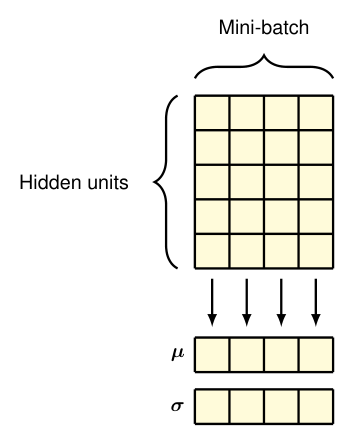
\includegraphics[width=0.4\textwidth]{figure7-8-b.png}
    \caption{图7-8-b: 层归一化：对该层（所有？）隐藏单元根据某个数据点进行归一化}
\end{figure}

\begin{table}[htbp]
    \centering
    \caption{输入归一化、批归一化与层归一化的核心对比}\vspace{0.2cm}
    \label{tab:normalization_comparison}
    \renewcommand{\arraystretch}{1.3} % 增加行高，使表格更美观
    \begin{tabular}{|p{3cm}|p{3cm}|p{3cm}|p{3cm}|} \hline 
        \textbf{对比维度} & \textbf{输入归一化} & \textbf{批归一化} & \textbf{层归一化} \\ \hline 
        \textbf{归一化对象} & 输入层的特征 & 隐藏层的预激活值 & 隐藏层的预激活值 \\ \hline 
        \textbf{归一化方向} & 跨所有样本\newline 对每个特征 & 跨小批量内的样本，对每个隐藏单元 & 跨隐藏单元，对每个数据点 \\ \hline 
        \textbf{计算时机} & 训练前一次性计算 & 训练时每个小批量动态计算 & 训练时每个数据点动态计算 \\ \hline 
        \textbf{可学习参数} & 无 & $\beta_i$（均值）、$\gamma_i$（标准差） & $\beta_i$（均值）、$\gamma_i$（标准差） \\ \hline 
        \textbf{推理阶段处理} & 使用固定的均值和方差 & 使用训练期间记录的移动平均值 & 与训练阶段完全相同，无需额外处理 \\ \hline 
        \textbf{是否需要移动平均} & 否 & 是 & 否 \\ \hline 
        \textbf{对小批量的依赖} & 否 & 是（批量越小，估计越不稳定） & 否 \\ \hline 
        \textbf{典型应用场景} & 几乎所有神经网络的数据预处理 & CNN 等前馈网络 & RNN、Transformer 等序列模型 \\ \hline 
    \end{tabular}
\end{table}

}

\end{document}